% pdflatex local.tex && pdflatex local.tex && del local.out, local.log, local.aux, local.toc && start local.pdf
\documentclass[a4paper, 12pt]{article}
\usepackage[T2A,T1]{fontenc}
\usepackage[utf8]{inputenc}
\usepackage[english, ukrainian]{babel}
\usepackage{amsmath, amssymb}
\allowdisplaybreaks
\setlength\parindent{0pt}
\numberwithin{equation}{section}% reset equation counter for sections
\title{{\Huge ОСНОВИ МЕТОДІВ ОБЧИСЛЕНЬ}}
\author{Нікіта Скибицький}
\date{\today}
\usepackage{xcolor}
\usepackage{hyperref}
\hypersetup{unicode=true,colorlinks=true,linktoc=all,linkcolor=red}
\usepackage{float, graphicx}
\usepackage{amsthm}
\newtheorem{lemma}{Лема}
\newtheorem*{lemma*}{Лема}
\newtheorem{theorem}{Теорема}[subsection]
\newtheorem*{theorem*}{Теорема}
\newtheorem{definition}{Визначення}
\newtheorem*{definition*}{Визначення}
\theoremstyle{definition}
\newtheorem{remark}{Зауваження}
\newtheorem*{remark*}{Зауваження}
\newtheorem{example}{Приклад}
\newtheorem*{example*}{Приклад}
\newtheorem{problem}{Задача}
\newtheorem*{problem*}{Задача}
\newtheorem{solution}{Розв'язок}
\newtheorem*{solution*}{Розв'язок}
\newtheorem{corollary}{Наслідок}
\newtheorem*{corollary*}{Наслідок}
\newcommand{\RR}{\mathbb{R}}
\newcommand{\CC}{\mathbb{C}}
\newcommand{\Min}{\displaystyle\min\limits}
\newcommand{\Max}{\displaystyle\max\limits}
\newcommand{\Inf}{\displaystyle\inf\limits}
\newcommand{\Sup}{\displaystyle\sup\limits}
\newcommand{\Sum}{\displaystyle\sum\limits}
\newcommand{\Prod}{\displaystyle\prod\limits}
\newcommand{\Int}{\displaystyle\int\limits}
\newcommand{\Iint}{\displaystyle\iint\limits}
\newcommand{\Lim}{\displaystyle\lim\limits}
\newcommand*\diff{\mathop{}\!\mathrm{d}}
\renewcommand{\bf}[1]{\textbf{#1}}
\renewcommand{\epsilon}{\varepsilon}
\renewcommand{\phi}{\varphi}
\DeclareMathOperator{\diam}{diam}
\DeclareMathOperator{\diag}{diag}
\DeclareMathOperator{\signum}{sign}
\DeclareMathOperator{\rang}{rang}
\DeclareMathOperator{\const}{const}
\DeclareMathOperator{\cond}{cond}
\begin{document}
\maketitle \thispagestyle{empty} \newpage 
У ваших руках конспект лекцій з нормативного курсу ``Основи методів обчислень'', прочитаного доц., к.ф.-м.н. Риженком Андрієм Івановичем на третьому курсі спеціальності прикладна математика факультету комп'ютерних наук та кібернетики Київського національного університету імені Тараса Шевченка восени 2018-го року. \\

Конспект у компактній формі відображає матеріал курсу, допомагає сформувати загальне уявлення про предмет вивчення, правильно зорієнтуватися в даній галузі знань. Конспект лекцій з названої дисципліни сприятиме більш успішному вивченню дисципліни, причому більшою мірою для студентів заочної форми, екстернату, дистанційного та індивідуального навчання. \\

Комп'ютерний набір та верстка -- Скибицький Нікіта Максимович. \newpage
\tableofcontents \newpage
\section{Аналіз похибок заокруглення}

\subsection{Види похибок}

Нехай необхідно розв’язати рівняння
\begin{equation}
	\label{eq:1.1}
	Au = f.
\end{equation}
За рахунок неточно заданих вхідних даних насправді ми маємо рівняння
\begin{equation}
	\label{eq:1.2}
	\tilde A \tilde u = \tilde f.
\end{equation}
Назвемо $\delta_1 = u - \tilde u$ -- \textit{неусувною похибкою}. \\

Застосування методу розв‘язання \eqref{eq:1.2} приводить до рівняння
\begin{equation}
	\label{eq:1.3}
	\tilde A_h \tilde u_h = \tilde f_h,
\end{equation}
де $h > 0$ -- малий параметр. Назвемо $\delta_2 \tilde u - \tilde u_h$ -- \textit{похибкою методу}. \\

Реалізація методу на ЕОМ приводить до рівняння
\begin{equation}
	\label{eq:1.4}
	\tilde A_h^* \tilde u_h^* = \tilde f_h^*.
\end{equation}
Назвемо $\delta_3 = \tilde u_h^* - \tilde u_h$ -- \textit{похибкою заокруглення}. \\

Тоді \textit{повна похибка} $\delta = u - \tilde u_h^* = \delta_1 + \delta_2 + \delta_3$. \\

\begin{definition}
	Кажуть, що задача \eqref{eq:1.1} \textit{коректна}, якщо
	\begin{enumerate}
		\item $\forall f \in F$ $\exists! u \in U$;
		\item задача \eqref{eq:1.1} \textit{стійка}, тобто
		\begin{equation}
			\label{eq:1.5}
			\forall \epsilon > 0 \quad \exists \delta > 0: \|A-\tilde A\| < \delta, \|f-\tilde f\| < \delta \Rightarrow \|u - \tilde u\| < \epsilon.
		\end{equation}
	\end{enumerate}
\end{definition}

Якщо задача \eqref{eq:1.1} \textit{некоректна}, то або розв‘язок її не існує, або він неєдиний, або він нестійкий, тобто 
\begin{equation}
	\label{eq:1.6}
	\exists \epsilon > 0: \forall \delta > 0: \exists A, f: \| A - \tilde A\|<\delta, \|f-\tilde f\| < \delta, \|u-\tilde u\| > \epsilon.
\end{equation}

\textit{Абсолютна похибка} $\Delta (x^*) \ge \max_x |x - x^*|$. \\

\textit{Відносна похибка} $\delta (x^*) \ge \max_x \Delta (x^*) / |x^*|$. \\

\textit{Значущими цифрами} називаються всі цифри, починаючи з першої ненульової зліва. \\

\textit{Вірна цифра} -- це значуща, якщо абсолютна похибка за рахунок відкидання всіх молодших розрядів не перевищує одиниці розряду цієї цифри. Тобто, якщо 
\begin{equation}
	\label{eq:1.7}
	x^* = \overline{\alpha_n \ldots \alpha_0.\alpha_{-1}\ldots\alpha_{-p}\ldots},
\end{equation}
то $\alpha_{-p}$ -- вірна, якщо $\Delta (x^*) \le 10^{-p}$. \\

Інколи $\Delta (x^*) \le w \cdot 10^{-p}$, $1/2 \le w < 1$, наприклад, $w = 0.55$.

\subsection{Підрахунок похибок в ЕОМ}

Підрахуємо відносну похибку заокруглення числа $x$ на ЕОМ з плаваючою комою. В $\beta$-ічній системі числення число представляється у вигляді
\begin{equation}
	\label{eq:1.8}
	x = \pm (\alpha_1 \beta^{-1} + \alpha_2 \beta^{-2} + \ldots + \alpha_t \beta^{-t} + \ldots) \beta^p,
\end{equation}
де $0 \le \alpha_k < \beta$, $\alpha_1 \ne 0$, $k = 1,2,\ldots$ \\

Якщо в ЕОМ $t$ розрядів, то при відкиданні молодших розрядів ми оперуємо з наближеним значенням 
\begin{equation}
	\label{eq:1.9}
	x^* = \pm (\alpha_1 \beta^{-1} + \alpha_2 \beta^{-2} + \ldots + \alpha_t \beta^{-t}) \beta^p,
\end{equation}
і відповідно похибка заокруглення 
\begin{equation}
	\label{eq:1.9_1}
	x - x^* = \pm \beta^p (\alpha_{t+1} \beta^{-t-1} + \ldots)
\end{equation}
Тоді її можна оцінити так
\begin{multline}
	\label{eq:1.10}
	|x - x^*| \le \beta^{p-t-1} \cdot (\beta-1) \cdot (1 + \beta^{-1}+\ldots)\le\\
	\le \beta^{p-t-1} \cdot (\beta-1) \cdot \dfrac{1}{1-\beta^{-1}}=\beta^{p-t}.
\end{multline}

Якщо в представлені \eqref{eq:1.8} взяти $\alpha_1 = 1$, то $|x| \ge \beta^p \cdot \beta^{-1}$. Звідси остаточно 
\begin{equation}
	\label{eq:1.11}
	\delta (x^*) \le \dfrac{\beta^{p-t}}{\beta^{p-1}}=\beta^{1-t}.
\end{equation}

При більш точних способах заокруглення можна отримати оцінку $\delta (x^*) \le \beta^{1-t} / 2 = \epsilon$. Число $\epsilon$ називається ``машинним іпсилон''. Наприклад, для $\beta = 2$, $t = 24$, $\epsilon = 2^{-24} \approx 10^{-7}$.

\subsection{Підрахунок похибок обчислення значення функції}

Нехай задана функція 
\begin{equation}
	\label{eq:1.11_1}
	y = f(x_1, \ldots, x_n) \in C^1(\Omega)
\end{equation}
Необхідно обчислити її значення при наближеному значенні аргументів 
\begin{equation}
	\label{eq:1.11_2}
	\vec x^* = (x_1^*, \ldots, x_n^*),
\end{equation}
де $|x_i - x_i^*| \le \Delta (x_i^*)$ та оцінити похибку обчислення значення функції
\begin{equation}
	\label{eq:1.11_3}
	y^* = f(x_1^*, \ldots, x_n^*).
\end{equation}

Маємо 
\begin{equation}
	\label{eq:1.12}
	|y-y^*| = |f\left(\vec x\right) - f\left(\vec x^*\right)| = \left| \Sum_{i=1}^n \dfrac{\partial f}{\partial x_i} \left(\vec \xi\right) (x_i - x_i^*) \right| \le \Sum_{i=1}^n B_i \cdot \Delta (x_i^*), 
\end{equation}
де 
\begin{equation}
	\label{eq:1.13}
	B_i = \Max_{\vec x \in U} \left| \dfrac{\partial f}{\partial x_i}\left(\vec x\right) \right|.
\end{equation}

Тут 
\begin{equation}
	\label{eq:1.14}
	U = \left\{ \vec x = (x_1, \ldots, x_n): |x_i - x_i^*| \le \Delta (x_i^*)\right\} \in \Omega, \quad i=\overline{1,n}.
\end{equation}
Отже
\begin{equation}
	\label{eq:1.15}
	\Delta (y^*) = |y - y^*| \prec \Sum_{i=1}^n n_i \cdot \Delta (x_i^*),
\end{equation}
з точністю до величин першого порядку малості по
\begin{equation}
	\label{eq:1.15_1}
	\Delta (x^*) = \Max_{i=\overline{1,n}} \Delta (x_i^*),
\end{equation}
де
\begin{equation}
	\label{eq:1.16}
	b_i = \left| \dfrac{\partial f}{\partial x_i}\left(\vec x^*\right) \right|
\end{equation}
та ``$\prec$'' означає приблизно менше. \\

\subsubsection{Похибки арифметичних операцій}

\begin{enumerate}
	\item Сума: $y = x_1 + x_2$, $x_1, x_2 > 0$, 
	\begin{equation}
		\label{eq:1.17}
		\begin{aligned}
		\Delta (y^*) &\le \Delta (x_1^*) + \Delta (x_2^*), \\ 
		\delta (y^*) &\le \dfrac{\Delta (x_1^*) + \Delta (x_2^*)}{x_1^* + x_2^*} \le \max\{\delta (x_1^*), \delta (x_2^*)\}.
		\end{aligned}
	\end{equation}
	
	\item Різниця: $y = x_1 - x_2$, $x_1 > x_2 > 0$,
	\begin{equation}
		\label{eq:1.18}
		\begin{aligned}
		\Delta (y^*) &\le \Delta (x_1^*) + \Delta (x_2^*), \\
		\delta (y^*) &\le \dfrac{x_2^* \delta (x_1^*) + (x_1^*) \delta (x_2^*)}{x_1^* - x_2^*}.
		\end{aligned}
	\end{equation}
	
	При близьких $x_1^*$, $x_2^*$ зростає відносна похибка (за рахунок втрати вірних цифр).

	\item Добуток: $y = x_1 \cdot x_2$, $x_1, x_2 > 0$,
	\begin{equation}
		\label{eq:1.19}
		\begin{aligned}
		\Delta (y^*) &\prec x_2^* \Delta (x_1^*) + x_1^* \Delta (x_2^*), \\
		\delta (y^*) &\le \delta (x_1^*) + \delta (x_2^*).
		\end{aligned}
	\end{equation}

	\item Частка: $y = \dfrac{x_1}{x_2}$, $x_1, x_2 > 0$,
	\begin{equation}
		\label{eq:1.20}
		\begin{aligned}
		\Delta (y^*) &\prec \dfrac{x_2^* \Delta (x_1^*) + x_1^* \Delta (x_2^*)}{(x_2^*)^2}, \\
		\delta (y^*) &\le \delta (x_1^*) + \delta (x_2^*).
		\end{aligned}
	\end{equation}

	При малих $x_2^*$ зростає абсолютна похибка (за рахунок зростання результату ділення). 
\end{enumerate}

\subsection{Обернена задача аналізу позибок}

Нагадаємо, що \textit{пряма задача} аналізу похибок полягає у обчисленні $\Delta (y^*), \delta (y^*)$ по заданих $\Delta (x_i^*)$, $i = \overline{1, n}$. \\

\textit{Обернена задача} полягає у знаходженні $\Delta (x_i^*)$, $i = \overline{1, n}$ по заданих $\Delta (y^*)$, $\delta (y^*)$. Якщо $n > 1$, маємо одну умову 
\begin{equation}
	\label{eq:1.21}
	\Sum_{i=1}^n b_i \Delta (x_i^*) < \epsilon
\end{equation}
для багатьох невідомих $\Delta (x_i^*)$. Вибирають їх із однієї з умов 
\begin{equation}
	\label{eq:1.22}
	b_i \Delta (x_i^*) < \dfrac{\epsilon}{n},
\end{equation}
або
\begin{equation}
	\label{eq:1.23}
	\Delta (x_i^*) < \dfrac{\epsilon}{\Sum_{i=1}^n b_i}.
\end{equation}
\section{Нелінійні рівняння}

\textit{Постановка задачі}. Нехай маємо рівняння $f(x) = 0$, $\overline{x}$ -- його розв’язок, тобто $f (\overline{x}) \equiv 0$. \\

Задача розв‘язання цього рівняння розпадається на етапи:
\begin{enumerate}
	\item Існування та кількість коренів.
	\item Відділення коренів, тобто розбиття числової вісі на інтервали, де знаходиться один корінь.
	\item Обчислення кореня із заданою точністю $\epsilon$.
\end{enumerate}

Для розв'язання перших двох задач використовуються методи математичного аналізу та алгебри, а також графічний метод. Далі розглядаються методи розв'язання третього етапу.

\subsection{Метод ділення навпіл}

Припустимо на $[a, b]$ знаходиться лише один корінь рівняння 
\begin{equation}
	\label{eq:2.1}
	f(x) = 0,
\end{equation}
для $f(x) \in C([a,b])$, який необхідно визначити. Нехай $f(a) \cdot f (b) < 0$. \\

Припустимо, що $f(a) > 0$, $f(b) < 0$. Покладемо $x_1 = \frac{a + b}{2}$ і підрахуємо
$f(x_1)$. Якщо $f_1(x) < 0$, тоді шуканий корінь $x$ знаходиться на інтервалі $(a, x_1)$. Якщо ж $f_1(x) > 0$, то $\overline{x} \in (x_1, b)$, тобто з двох інтервалів $(a, x_1)$ і $(x_1, b)$ вибираємо той, на границях якого функція $f(x)$ має різні знаки, знаходимо точку $x_2$ -- середину вибраного інтервалу, підраховуємо $f(x_2)$ і повторюємо вказаний процес. \\

В результаті отримаємо послідовність інтервалів, що містять шуканий корінь $\overline{x}$, причому довжина кожного послідуючого інтервалу вдвічі менше попереднього. \\

Цей процес продовжується до тих пір, поки довжина отриманого інтервалу $(a_n, b_n)$ не стане меншою за $b_n - a_n < 2 \epsilon$. Тоді $x_{n+1}$, як середина інтервалу $(a_n, b_n)$ пов'язане з $\overline{x}$ нерівністю
\begin{equation}
	\label{eq:2.2}
	|x_n+1 - \overline{x}| < \epsilon.
\end{equation}

Ця умова для деякого $n$ буде виконуватись за теоремою Больцано-Коші. \\

Оскільки
\[ |b_{k + 1} - a_{k + 1} | = \dfrac12 |b_k - a_k|, \]
то
\begin{equation}
	\label{eq:2.3}
	|x_{n+1} - \overline{x}| \le \dfrac{1}{2^{n+1}} (b - a) < \epsilon.
\end{equation}

Звідси отримаємо нерівність для обчислення кількості ітерацій $n$ для виконання умови (\ref{eq:2.2}):
\[ n = n(\epsilon) \ge \left\lfloor \log\left(\dfrac{b-a}{\epsilon}\right) \right\rfloor + 1. \]

Степінь збіжності -- лінійна, тобто геометричної прогресії з знаменником $q = \frac12$. \\

Переваги методу: простота, надійність. Недоліки методу: низька швидкість збіжності; метод не узагальнюється на системи. 

\subsection{Метод простої ітерації}

Спочатку рівняння
\begin{equation}
	\label{eq:2.4}
	f (x) = 0
\end{equation}
замінюється еквівалентним
\begin{equation}
	\label{eq:2.5}
	x = \phi(x)
\end{equation}
Ітераційний процес має вигляді
\begin{equation}
	\label{eq:2.6}
	x_{n+1} = \phi(x_n), \quad n = 0,1,\ldots
\end{equation}

Початкове наближення $x_0$ задається. \\

Для збіжності велике значення має вибір функції $\phi(x)$. Перший спосіб заміни рівняння полягає в відділенні змінної з якогось члена рівняння. Більш продуктивним є перехід від рівняння (\ref{eq:2.4}) до (\ref{eq:2.5}) з функцією $\phi (x) = x + \tau (x) \cdot f (x)$, де $\tau (x)$ -- знакостала функція на тому відрізку, де шукаємо корінь. \\

Кажуть, що ітераційний метод \textit{збігається}, якщо $\Lim_{k\to\infty} x_k = \overline{x}$. \\

Далі $U_r = \{x : |x - a| \le r\}$ відрізок довжини $2r$ з серединою в точці $a$. \\

З'ясуємо умови, при яких збігається метод простої ітерації.

\begin{theorem}
	Якщо $\Max_{x \in U_r} |\phi'(x)| \le q < 1$, то метод простої ітерації збігається і має місце оцінка 
	\begin{equation}
		\label{eq:2.7}
		|x_n - \overline{x}| \le \dfrac{q^n}{1-q}|x_0-x_1| \le \dfrac{q^n}{1-q}(b-a).
	\end{equation}
\end{theorem}

\begin{proof}
	Нехай $x_{k+1}, x_k \in U_r$. Тоді має місце допоміжна нерівність:
	\begin{multline*}
		|x_{k+1} - x_k| = |\phi(x_k) - \phi(x_{k-1})| = |\phi'(\xi_k)(x_k - x_{k-1}) \le (*) \\
		\text{тут }\xi_k = x_k + \theta_k (x_{k+1} - x_k), \quad 0 < \theta_k < 1 \\
		(*) \le |\phi'(\xi_k)| \cdot |x_k - x_{k-1}| \le q |x_k - x_{k-1}| = \ldots = q^k |x_1 - x_0|.
	\end{multline*}
	Використаємо її для доведення теореми:
	\begin{multline}
		\label{eq:2.8}
		|x_{k+p} - x_k| = |x_{k+p} - x_{k+p-1} + \ldots + x_{k+1} - x_k| \le \\
		\le |x_{k+p} - x_{k+p-1}| + \ldots + |x_{k+1} - x_k| \le \\
		\le (q^{k+p-1}+q^{k+p-2}+\ldots+q^k) |x_1 - x_0| = \\
		= \dfrac{q^k - q^{k+p-1}}{1-q}|x_1-x_0| \xrightarrow[k\to\infty]{}0.
	\end{multline}

	Бачимо що $\{x_k\}$ -- фундаментальна послідовність. Значить вона збіжна. При $p\to\infty$ в (\ref{eq:2.8}) отримуємо (\ref{eq:2.7}).
\end{proof}

Визначимо кількість ітерацій для досягнення точності $\epsilon$. З оцінки в теоремі отримаємо \[ |x_n - \overline{x}| \le \dfrac{q^n}{1-q}(b-a) < \epsilon \Rightarrow n(\epsilon) = n \ge \left\lfloor \dfrac{\ln \left(\dfrac{\epsilon (1-q)}{b - a}\right)}{\ln q} \right\rfloor + 1. \]

Практично ітераційний процес зупиняємо при: $|x_n - x_{n-1}| < \epsilon$. Але ця умова не завжди гарантує, що $|x_n - \overline{x}| < \epsilon$.

\begin{remark*}
	Умова збіжності методу може бути замінена на умову Ліпшиця \[|\phi(x) -\phi(y)| \le q \cdot| x - y |,\quad 0 < q < 1.\]
\end{remark*}

Переваги методу: простота; при $q < \frac12$ -- швидше збігається ніж метод ділення навпіл; метод узагальнюється на системи. Недоліки методу: 
\begin{enumerate}
	\item при $q > \frac12$ -- збігається повільніше ніж метод ділення навпіл,
	\item виникають труднощі при зведенні $f (x) = 0$ до $x =\phi (x)$.
\end{enumerate}


\subsection{Метод релаксації}

Якщо в методі простої ітерації для рівняння $x = x +\tau f (x) \equiv\phi (x)$ вибрати $\tau (x) =\tau = \const$, то ітераційний процес приймає вигляд
\begin{equation}
	\label{eq:2.9}
	x_{n+1} = x_n +\tau \cdot f(x_n), \quad n = 0,1,2,\ldots
\end{equation}
$x_0$ -- задано. Метод можна записати у вигляді \[\dfrac{x_{k+1}-x_k}{\tau} = f(x_k), \quad k=0,1,\ldots.\] Оскільки $\phi'(x) =1+\tau\cdot f'(x)$, то метод збігається при умові \[ |\phi'(x)| = |1+\tau \cdot f'(x)| \le q < 1.\]

Нехай $f'(x) < 0$, тоді (\ref{eq:2.7}) запишеться у вигляді: $-q \le 1 +\tau \cdot f'(x) \le q < 1$. Звідси \[\tau \cdot |f'(x_k)| \le 1 + q < 2 \quad \text{і} \quad 0 < \tau < \dfrac{2}{|f'(x)|}. \]

Поставимо задачу знаходження $\tau$, для якого $q = q(\tau) \to \min$. Для того, щоб вибрати оптимальний параметр $\tau$, розглянемо рівняння для похибки $z_k = x_j - \overline{x}$. \\

Підставивши $x_k = x + z_k$ в (\ref{eq:2.9}), отримаємо
\[ z_{k+1} = z_k + \tau \cdot f(\overline{x} + z_k).\]

В припущені $f(x)\in C^{(1)}([a,b])$ з теореми про середнє маємо
\[ f(\overline{x} + z_k) = f(\overline{x}) + z_k \cdot f'(\overline{x} + \theta z_k) = z_k \cdot f'(\overline{x}+\theta z_k) = z_k \cdot f'(\xi_k), \]
\[ z_{k+1} = z_k + \tau \cdot f'(\xi_k) \cdot z_k, \]
\[ |z_{k+1}| \le |1 + \tau \cdot f'(\xi_k)| \cdot |z_k| \le \Max_{\xi_k \in U} |1 + \tau \cdot f'(\xi_k)| \cdot |z_k|, \]
\[ |z_{k+1}| \le \max \{|1-\tau \cdot M_1|, |1-\tau \cdot m_1| \}\cdot |z_k|, \]
\[ m_1 = \Min_{x\in[a,b]} |f'(x)|, \quad M_1 = \Max_{x\in[a,b]} |f'(x)|. \]

Таким чином, задача вибору оптимального параметра зводиться до знаходження $\tau$, для якого функція \[ q(\tau) = \max\{|1-\tau \cdot M_1|,|1-\tau \cdot m_1|\}\]
приймає мінімальне значення: $q(\tau)\to\min$.

\begin{figure}[H]
	\centering
	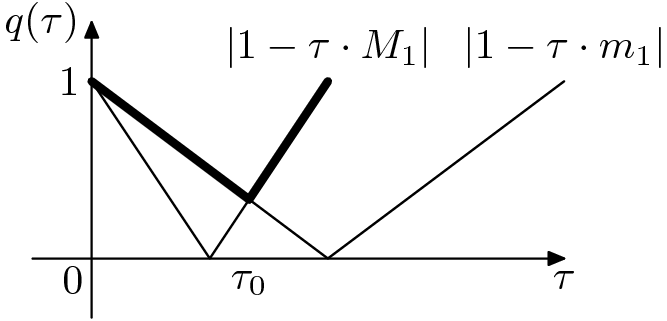
\includegraphics[width=.5\linewidth]{mal-1.png}
\end{figure}

% u:=1cm;
% label.llft(btex $0$ etex, (0,0));
% label.lft(btex $1$ etex, (0,3u/2));
% drawarrow (-u/2,0)--(4u,0);
% drawarrow (0,-u/2)--(0,2u);
% label.lft(btex $q(\tau)$ etex, (0,2u));
% label.bot(btex $\tau$ etex, (4u,0));
% draw (0,3u/2)--(u,0)--(2u,3u/2);
% draw (0,3u/2)--(2u,0)--(4u,3u/2);
% label.top(btex $|1-\tau \cdot M_1|$ etex, (2u,3u/2));
% label.top(btex $|1-\tau \cdot m_1|$ etex, (4u,3u/2));
% draw (4/3u,u/2)--(2u,3u/2) withpen pencircle scaled 2bp;
% draw (0,3u/2)--(4/3u,u/2) withpen pencircle scaled 2bp;
% label.bot(btex $\tau_0$ etex, (4/3u,0));

З графіка видно, що точка мінімуму визначається умовою $|1 - \tau \cdot M_1| = |1 - \tau \cdot m_1|$. \\

Тому
\[ 1 - \tau_0 \cdot m_1 = \tau_0 \cdot M_1 - 1 \Rightarrow \tau_0 = \dfrac{2}{M_1+m_1} < \dfrac{2}{|f'(x)|}.\]

При цьому значенні $\tau$ маємо \[q(\tau_0) = q_0 =\dfrac{M_1-m_1}{M_1+m_1}.\]

Тоді для похибки вірна оцінка \[|x_n-\overline{x}|\le \dfrac{q_0^n\cdot (b-a)}{1-q_0}<\epsilon.\]

Кількість ітерацій \[n = n(\epsilon) \ge \left\lfloor \dfrac{\ln \left(\dfrac{\epsilon\cdot(1-q_0)}{b-a}\right)}{\ln q_0} \right\rfloor + 1.\]	

\begin{problem} 
	Дати геометричну інтерпретацію методу простої ітерації для випадків:
	\[ 0 < \phi'(x) < 1; \quad -1 < \phi'(x) < 0; \quad \phi'(x) < -1; \quad \phi'(x) > 1,\]
\end{problem}

\begin{problem} 
	Знайти оптимальне $\tau = \tau_0$ для методу релаксації при $f'(x) > 0$.
\end{problem}

\subsection{Метод Ньютона (метод дотичних)}

Припустимо, що рівняння $f (x) = 0$ має простий дійсний корінь $\overline{x}$, тобто $f (\overline{x}) = 0$, $f'(\overline{x}) \ne 0$. Нехай виконуються умови: $f (x)\in C^{(1)}([a,b])$, $f (a)\cdot f (b) < 0$. Тоді 
\[0 = f (\overline{x}) = f (x_k + \overline{x} - x_k ) = f (x_k ) + f'(\xi_k ) \cdot (\overline{x} - x_k ),\] 
де $\xi_k=x_k+\theta_k \cdot (\overline{x}-x_k)$, $0 < \theta_k < 1$, $\xi_k \approx x_k$. Тому наступне наближення виберемо з рівняння 
\[ f(x_k) + f'(x_k) \cdot (x_{k+1}-x_k) = 0.\]

Звідси маємо ітераційний процес
\[ x_{k+1} = x_k - \dfrac{f(x_k)}{f'(x_k)}, \quad k = 0,1,2,\ldots, \quad x_0\text{ -- задане}. \]

Метод Ньютона ще називають методом лінеаризації або методом дотичних.

\begin{problem} 
	Дати геометричну інтерпретацію методу Ньютона.
\end{problem}

Метод Ньютона можна інтерпретувати як метод простої ітерації з \[ \phi(x) = x - \dfrac{f(x)}{f'(x)}, \quad \text{тобто} \quad \tau(x) = - \dfrac{1}{f'(x)}. \]

Тому 
\[ \phi'(x) = 1 - \dfrac{f'(x)\cdot f'(x)-f(x)\cdot f''(x)}{(f'(x))^2} = \dfrac{f(x)\cdot f''(x)}{(f'(x))^2}.\]
Якщо $\overline{x}$ -- корінь $f(x)$, то $\phi'(x) = 0$. Тому знайдеться окіл кореня, де \[ |\phi'(x)| = \left|\dfrac{f(x)\cdot f''(x)}{(f'(x))^2}\right|<1.\]

Це означає, що збіжність методу Ньютона залежить від вибору $x_0$. \\

Недолік методу Ньютона: необхідність обчислювати на кожній ітерації не тільки значення функції, а й похідної. \\

Модифікований метод Ньютона позбавлений цього недоліку і має вигляд:
\[ x_{k+1} = x_k - \dfrac{f(x_k)}{f'(x_0)}, \quad k=0,1,2,\ldots. \]

Цей метод має лише лінійну збіжність: $|x_{k+1} - \overline{x}| = O(|x_k-\overline{x}|)$.
\begin{problem} 
	Дати геометричну інтерпретацію модифікованого методу Ньютона.
\end{problem}

В методі Ньютона, для якого $f'(x_k)$ замінюється на $\frac{f(x_k)-f(x_{k-1})}{x_k-x_{k-1}}$ дає метод січних: \[ x_{k+1} = x_k - \dfrac{x_k-x_{k-1}}{f(x_k)-f(x_{k-1})}\cdot f(x_k), \quad k = 1,2,\ldots, \quad x_0,x_1\text{ -- задані}.\]

\begin{problem} 
	Дати геометричну інтерпретацію методу січних.
\end{problem}

\subsection{Збіжність методу Ньютона}

\begin{theorem}
	Нехай $f(x)\in C^{(2)}([a,b])$, $\overline{x}$ -- простий дійсний корінь рівняння
	\begin{equation}
		\label{eq:2.10}
		f (x) = 0
	\end{equation}
	і $f'(x) \ne 0$ при $x\in U_r= \{x: |x -\overline{x}| < r\}$. Якщо
	\begin{equation}
		\label{eq:2.11}
		\dfrac{M_2\cdot|x_0-\overline{x}|}{2m_1} = q < 1
	\end{equation}
	де $m_1 = \Min_{x\in U_r} |f'(x)|$, $M_2 = \Max_{x\in U_r} |f''(x)|$, то для $x_0 \in U_r$ метод Ньютона 
	\begin{equation}
		\label{eq:2.12}
		x_{k+1} = x_k - \dfrac{f(x_k)}{f'(x_k)}
	\end{equation}
	збігається і має місце оцінка
	\begin{equation}
		\label{eq:2.13}
		|x_n - \overline{x}| \le q^{2^n-1} \cdot |x_0 - \overline{x}|.
	\end{equation}
\end{theorem}

\begin{proof}
	З (\ref{eq:2.12}) маємо 
	\begin{equation}
		\label{eq:2.14}
		x_{k+1} - \overline{x} = x_k - \dfrac{f(x_k)}{f'(x_k)} - \overline{x} = \dfrac{(x_k-\overline{x}) \cdot f'(x_k)-f(x_k)}{f'(x_k)} = \dfrac{F(x_k)}{f'(x_k)},
	\end{equation}
	де $F(x) = (x - \overline{x}) \cdot f'(x) - f (x)$, така, що
	\begin{enumerate}
		\item $F(x) = 0$;
		\item $F'(x) = (x - \overline{x}) \cdot f''(x)$;
	\end{enumerate}
	Тоді \[ F(x_k) = F(\overline{x}) + \Int_{\overline{x}}^{x_k}  F'(t) \diff t = \Int_{\overline{x}}^{x_k}  ((t - \overline{x}) \cdot f''(t)) \diff t . \]

	Так як $(t - x)$ не міняє знак на відрізку інтегрування, то скористаємося теоремою про середнє значення:
	\begin{equation}
		\label{eq:2.15}
		F(x_k) = f''(\xi_k) \Int_{\overline{x}}^{x_k}  (t - \overline{x}) \diff t = \dfrac{(x_k-\overline{x})^2}{2} f''(\xi_k),
	\end{equation}
	де $\xi_k = \overline{x} + \theta_k \cdot (x_k - \overline{x})$, $0 <\theta_k < 1$. З (\ref{eq:2.14}), (\ref{eq:2.15}) маємо
	\begin{equation}
		\label{eq:2.16}
		x_{k+1} - \overline{x} = \dfrac{(x_k-\overline{x})^2}{2f'(x_k)} f''(\xi_k).
	\end{equation}
	Доведемо оцінку (\ref{eq:2.12}) за індукцією. Так як $x_0 \in U_r$, то \[|\xi_0 - \overline{x}| = |\theta_0 \cdot (x_0 - \overline{x})| < |\theta_0| \cdot |x_0 - \overline{x}| < r \Rightarrow \xi_0 \in U_r.\]

	Тоді $f''(\xi_0) \le M_2$, тому
	\begin{multline*} 
		|x_1 - \overline{x}| \le \dfrac{(x_0-\overline{x})^2 \cdot M_2}{2m_1} = \dfrac{M_2\cdot|x_0-\overline{x}|}{2m_1}|x_0-\overline{x}| = \\
		= q\cdot |x_0-\overline{x}|=q\cdot |x_0-\overline{x}|<r \Rightarrow x_1\in U_r.
	\end{multline*}

	Ми довели твердження (\ref{eq:2.13}) при $n = 1$. Нехай воно справджується при $n = k$:
	\[ |x_k - \overline{x}| \le q^{2^k-1}\cdot |x_0 - \overline{x}| < r, \quad |\xi_k - \overline{x}| = |\theta_k \cdot (x_k - \overline{x})| < r. \]

	Тоді $x_k, \xi_k \in U_r$. \\

	Доведемо (\ref{eq:2.13}) для $n = k +1$. З (\ref{eq:2.16}) маємо 
	\begin{multline*}
		|x_{k+1}-\overline{x}| \le \dfrac{|x_k - \overline{x}|^2\cdot M_2}{2m_1} \le \left(q^{2^k-1}\right)^2 \dfrac{|x_0-\overline{x}|^2\cdot M_2}{2m_1} = \\
		= q^{2^{k+1}-2} \dfrac{|x_0-\overline{x}|\cdot M_2}{2m_1}|x_0-\overline{x}| = q^{2^{k+1}-1} \cdot |x_0-\overline{x}|.
	\end{multline*}

	Таким чином (\ref{eq:2.13}) справджується для $n = k +1$. Значить (\ref{eq:2.13}) виконується і для довільного $n$. Таким чином $x_n \xrightarrow[n\to\infty]{} \overline{x}$.
\end{proof}

З (\ref{eq:2.13}) маємо оцінку кількості ітерацій для досягнення точності $\epsilon$:
\[ n \ge \left\lfloor\log_2\left(1+\dfrac{\ln \left(\dfrac{\epsilon}{b-a}\right)}{\ln q}\right) \right\rfloor + 1 .\]

Кажуть, що ітераційний метод має \textit{степінь збіжності} $m$, якщо \[ |x_{k+1}-\overline{x}|=O(|x_k-\overline{x}|^m).\]

Для методу Ньютона 
\[|x_{k+1}-\overline{x}| = \dfrac{|x_k-\overline{x}|^2\cdot|f''(\xi_k)|}{2|f'(x_k)|}| \Rightarrow |x_{k+1}-\overline{x}|=O(|x_k-\overline{x}|^2).\]

Значить степінь збіжності методу Ньютона $m=2$. Для методу простої ітерації і ділення навпіл $m=1$.

\begin{theorem}
	Нехай $f(x)\in C^{(2)}([a,b])$ та $\overline{x}$ -- простий корінь рівняння $f (x) = 0$ а також $\forall x\in[a,b]$: $f'(x) \ne 0$. Якщо $f'(x) \cdot f''(x) > 0$ ($f'(x) \cdot f''(x) < 0$) то для методу Ньютона при $x_0 = b$ послідовність наближень $\{x_k \}$ монотонно спадає (монотонно зростає при $x_0 = a$).
\end{theorem}

\begin{problem}
	Довести теорему при 
	\begin{enumerate}
		\item $f'(x) \cdot f''(x) > 0$;
		\item $f'(x) f''(x) < 0$.
	\end{enumerate}
\end{problem}

\begin{problem}
	Знайти степінь збіжності методу січних.
\end{problem}


Якщо $f(a) \cdot f''(a) > 0$ та $f''(x)$ не міняє знак, то потрібно вибирати $x_0 = a$; при цьому $\{x_k \}\uparrow \overline{x}$. \\

Якщо $f(b) \cdot f''(b) > 0$, то $x_0 = b$; маємо $\{x_k \}\downarrow \overline{x}$. Пояснення на рисунку:

% u := 1cm;
% drawarrow (-u/2, 0)--(4u, 0);
% drawarrow (0, -u/2)--(0, 2u);
% draw (u/2,0)--(u/2,u/8);
% draw (7u/2,0)--(7u/2,u/8);
% label.bot(btex $a$ etex, (u/2, 0));
% label.top(btex $b$ etex, (7u/2, u/8));
% draw (u/2,3u/2){dir -75}..(2u,-u/2){dir 0}..(7u/2,-u/4);
% label.top(btex $x_0 = a$ etex, (2u,u));

% u := 1cm;
% drawarrow (-u/2, 0)--(4u, 0);
% drawarrow (0, -u/2)--(0, 2u);
% draw (u/2,0)--(u/2,u/8);
% draw (7u/2,0)--(7u/2,u/8);
% label.top(btex $a$ etex, (u/2, u/8));
% label.bot(btex $b$ etex, (7u/2, 0));
% draw (u/2,-3u/7){dir 75}..(2u,u)..(7u/2,3u/2);
% label.top(btex $x_0 = a$ etex, (2u,3u/2));

\begin{figure}[H]
	\centering
	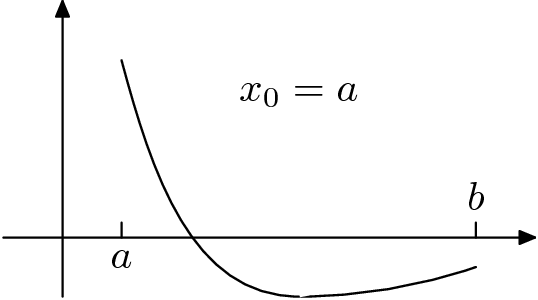
\includegraphics[width=.45\linewidth]{mal-2.png}
	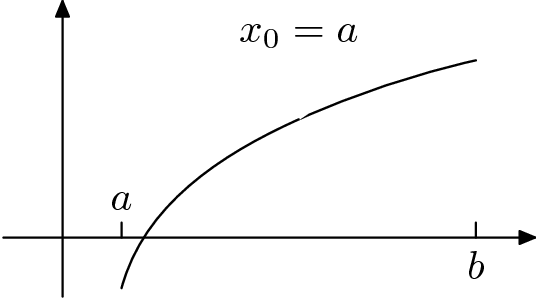
\includegraphics[width=.45\linewidth]{mal-3.png}
\end{figure}

\begin{remark}
	Якщо $\overline{x}$ -- $p$-кратний корінь тобто $f^{(m)} (x) = 0$, $m = \overline{0,p-1}$, $f^{ (p)} (x) \ne 0$, то в методі Ньютона необхідна наступна модифікація \[x_{k+1} = x_k - p\dfrac{f(x_k)}{f'(x_k)} \quad \text{і} \quad q = \dfrac{M_{p+1}\cdot|x_0-\overline{x}|}{m_p \cdot (p+1)}<1.\]
\end{remark}

\begin{remark}
Метод Ньютона можна застосовувати і для обчислення комплексного кореня, тоді ітераційний процес має вигляд \[z_{k+1} = z_k - \dfrac{f(z_k)}{f'(z_k)}, \quad k = 0,1,\ldots.\] В теоремі про збіжність $q = \frac{|z_0-\overline{z}|\cdot M_2}{2m_1}$, де $m_1 = \Min_{z\in U_r} |f'(z)|$, $M_2 = \Max_{z\in U_r} |f''(z)|$. Тут $|z|$ -- модуль комплексного числа $z$.
\end{remark}

Переваги методу Ньютона: 
\begin{enumerate}
\item висока швидкість збіжності;
\item узагальнюється на системи рівнянь; 
\item узагальнюється на комплексні корені.
\end{enumerate}
Недоліки методу Ньютона: 
\begin{enumerate}
	\item на кожній ітерації обчислюється не тільки $f (x_k )$ , а і похідна $f'(x_k)$;
	\item  збіжність залежить від початкового наближення $x_0$, так як від нього залежить умова збіжності $q = \frac{M_2\cdot |x_0-\overline{x}|}{2m_1} < 1$;
	\item потрібно, щоб $f (x)\in C^{(2)}([a,b])$.
\end{enumerate}
\subsubsection{Характеристики розсіювання значень}
Нехай маємо вибірку об'єму $n$ спостережень $x_1$, $x_2$, $\ldots$, $x_n$ над випадковою величиною $\xi$.
\begin{enumerate}
	\item \textit{Дисперсія} $D\xi = M(\xi - M\xi)^2$. Вибіркове значення \[ S^2(n) = \dfrac{1}{n-1} \sum_{i=1}^n (x_i - \bar{x}(n))^2 = \dfrac{1}{n-1} \left(\sum_{i=1}^n x_i^2 - n\bar{x}^2(n) \right). \]
	\item \textit{Стандартне (середньоквадратичне) відхилення} $\sqrt{D\xi}$. Вибіркове значення $S(n)$.
	\item \textit{Коефіцієнт варіацій} $V_\xi = \frac{\sqrt{D\xi}}{M\xi} 100\%$, $M\xi\ne0$. Вибіркове значення $\widehat{V}_\xi(n)=\frac{S(n)}{\bar x(n)} 100\%$.
	\item \textit{Стохастичне розсіювання} (імовірнісне відхилення) -- це половина інтерквартильної широти: $\frac{U_{0.75} - U_{0.25}}{2}$. Вибіркове значення $\frac{\widehat{U}_{0.75} - \widehat{U}_{0.25}}{2}$.
	\item \textit{Розмах (широта) вибірки}: $x_{\max}-x_{\min}$, де $x_{\max}, x_{\min}$ -- найбільше та найменше значення у вибірці.
	\item \textit{Інтервал концентрації} $(M\xi - 3\sqrt{D\xi}, M\xi + 3 \sqrt{D\xi})$. Вибіркове значення $(\bar x(n) - 3S(n), M\bar x(n) + 3 S(n))$.
\end{enumerate}
\subsubsection{Характеристики скошеності та гостроверхості розподілу}
Нехай є розподіл випадкової величини $\xi$ і отримані спостереження $x_1$, $x_2$, $\ldots$, $x_n$ над нею.
\begin{enumerate}
	\item \textit{Коефіцієнт асиметрії} -- характеристика скошеності розподілу (базується на третьому центральному моменті): \[ \beta_1 = \dfrac{M(\xi - M\xi)^3}{(M(\xi - M\xi)^2)^{3/2}}, \quad D\xi > 0. \] Вибіркове значення \[ \widehat{\beta}_1 = \dfrac{\dfrac{1}{n}\Sum_{i=1}^n(x_k - \bar{x}(n))^3}{S^3(n)}. \] Дисперсія спостережуваної величини $D\xi > 0$. \\ % figure 6

	Якщо розподіл симетричний (наприклад нормальний) то $\beta_1 =0$. Якщо $\beta_1 > 0$, то розподіл скошений вліво, якщо $\beta_1 < 0$, то вправо.
	\item \textit{Коефіцієнт ексцесу} -- характеристика гостроверхості розподілу (базується на четвертому центральному моменті): \[ \beta_2 = \dfrac{M(\xi-M\xi)^4}{(M(\xi-M\xi)^2)^2} - 3, \quad D\xi > 0. \] Вибіркове значення \[ \widehat{\beta}_2 = \dfrac{\dfrac{1}{n}\Sum_{i=1}^n(x_k - \bar{x}(n))^4}{S^4(n)} - 3. \]
	Для нормального розподілу коефіцієнт ексцесу дорівнює нулю. Якщо $\beta_2 > 0$, то розподіл більш гостроверхий ніж нормальний, якщо $\beta_2 < 0$ то відповідно менш гостроверхий.
\end{enumerate}
\subsection{Характеристики векторних величин}
Аналіз $q$-вимірних векторних величин, отримано $n$ спостережень над вектором $\vec\xi: x_1, x_2, \ldots, x_n$, $x_i \in \RR^q$, $i = \overline{1,n}$.
\subsubsection{Характеристики положення центру значень}
\begin{enumerate}
	\item \textit{Математичне сподівання} (теоретичне середнє) $M\xi$. Вибіркове значення \[\bar{x}(n) = \dfrac{1}{n} \Sum_{i=1}^n \vec{x}_i.\]
	\item \textit{Мода} $x_{\text{mod}}$. У неперервному випадку -- це точка максимуму функції щільності $\xi$. Для дискретного випадку -- це значення, яке набуває $\xi$ з найбільшою ймовірністю.
\end{enumerate}
\subsubsection{Характеристики розсіювання значень}
\begin{enumerate} 
	\item \textit{Коваріаційна матриця} $\sum = M(\xi - M\xi)(\xi - M\xi)^T$. Вибіркове значення \[\widehat{\sum}(n) = \dfrac{1}{n-1} \Sum_{k=1}^n (x_k - \bar x(n))(x_k - \bar x(n))^T.\]
	\item \textit{Узагальнена дисперсія} -- визначник коваріаційної матриці: $\det \sum$. Вибіркове значення $\det\left(\widehat{\sum}\right)$.
	\item \textit{Слід коваріаційної матриці} $\trace\sum$. Вибіркове значення $\trace\left(\widehat{\sum}(n)\right)$.
\end{enumerate}
\subsection{Перевірка стохастичності вибірки}
Перевіряємо, чи справді вибірка є випадковою, а не знаходиться під впливом деякого систематичного зміщення. Для цього запропоновано критерії:
\begin{itemize}
	\item Критерій серій на базі медіани
	\item Критерій зростаючих та спадаючих серій
	\item Критерій квадратів послідовних різниць (критерій Аббе)
\end{itemize}
Нехай $x_1$, $x_2$, $\ldots$, $x_n$ -- вибірка спостережень, яка досліджується. \\

Будемо перевіряти гіпотезу $H_0$: ця вибірка є стохастичною з рівнем значимості $\alpha (0 < \alpha < 1$) (рівень значимості -- ймовірність допустити помилку першого роду).
\begin{enumerate}
	\item \textit{Критерій серій на базі медіани}. Альтернативна гіпотеза $H_1$: наявність у вибірці систематичного монотонного зміщення середнього. \\

	Спочатку визначається вибіркове значення медіани $\widehat{x}_{\text{med}}$. Потім під кожним членом вибірки ставимо відповідно \[ \begin{cases} +, & x_i > \widehat{x}_{\text{med}} \\
 \text{нічого}, & x_i = \widehat{x}_{\text{med}} \\
 -, & x_i < \widehat{x}_{\text{med}} \end{cases}. \]
	Отримаємо послідовність символів. \textit{Серія} -- послідовність підряд розташованих однакових символів $+$ чи $-$. \textit{Довжина серії} -- це кількість членів у ній. \\

	Для отриманої послідовності обчислюємо дві статистики: загальну кількість серій в послідовності $v(n)$, довжину найдовшої серії $\tau(n)$. Запишемо область прийняття нашої гіпотези: \[ \left\{ \begin{matrix} v(n) > v_\beta(n) \\
 \tau(n) < \tau_{1-\beta}(n) \end{matrix} \right. \] 
	де $v_\beta(n)$, $\tau_\beta(n)$ -- квантилі рівня $\beta$ статистик $v(n)$, $\tau(n)$ відповідно. При фіксованому значенні $\beta$ рівень значимості $\alpha$ лежить у межах $\beta < \alpha < 2\beta - \beta^2$. Якщо порушується хоч одна з нерівностей, то гіпотеза відхиляється.
	\item \textit{Критерій зростаючих та спадаючих серій}. Альтернативна гіпотеза $H_1$: наявність у вибірці систематичного періодичного зміщення середнього. Спочатку у вибірці замінюємо підряд розташовані однакові виміри одним їх представником. В результаті отримаємо послідовність $x_1'$, $x_2'$, $\ldots$, $x_k'$. Під кожним членом послідовності ставимо відповідно \[ \begin{cases} +, & x_i' < x_{i+1}' \\
 -, & x_i' > x_{i+1}' \end{cases}. \]
	Далі для таким чином отриманої послідовності $+$ та $-$, як і в попередньому випадку, обчислюємо дві статистики: загальну кількість серій в послідовності $v(n)$, довжину найдовшої серії $\tau(n)$. Запишемо область прийняття нашої гіпотези: \[ \left\{ \begin{matrix} v(n) > v_\beta(n) \\
 \tau(n) < \tau_{1-\beta}(n) \end{matrix} \right. \] де $v_\beta(n)$, $\tau_\beta(n)$ -- квантилі рівня $\beta$ статистик $v(n)$, $\tau(n)$ відповідно. При фіксованому значенні $\beta$ рівень значимості $\alpha$ лежить у межах $\beta < \alpha < 2\beta - \beta^2$. Якщо порушується хоч одна з нерівностей, то гіпотеза відхиляється.
	\item \textit{Критерій квадратів послідовних різниць (критерій Аббе)}. Він є найбільш потужним на класі усіх нормальних вибірок. Альтернативна гіпотеза $H_1$: наявність у вибірці систематичного зміщення середнього. \\

	На основі вибірки підраховуємо наступну статистику: \[ \gamma(n) = \dfrac{\dfrac{1}{2(n-1)} \Sum_{i=1}^{n-1} (x_{i+1}-x_i)^2}{\dfrac{1}{n-1}\left(\Sum_{i=1}^n x_i^2 - n \bar{x}^2(n)\right)}. \]
	Область прийняття гіпотези для цього критерію має вигляд $\gamma(n) > \gamma_\alpha(n)$, де $\gamma_\alpha(n)$ -- квантиль рівня $\alpha$ статистики $\gamma(n)$, що при $n \le 60 $визначається з таблиць, а протилежному випадку потрібно скористатися формулою \[\gamma_\alpha(n) = 1 + \dfrac{u_\alpha}{\sqrt{n + 0.5(1 + u_\alpha^2)}}, \] де $u_\alpha$ -- квантиль рівня $\alpha$ нормального розподілу з параметрами 0 та 1.
\end{enumerate}
\section{Ітераційні методи для систем}

\subsection{Ітераційні методи розв'язання СЛАР}

Систему
\begin{equation}
	\label{eq:4.1}
	A \vec x = \vec b
\end{equation}
зводимо до вигляду
\begin{equation}
	\label{eq:4.2}
	\vec x = B \vec x + \vec f.
\end{equation}
Будь яка система
\begin{equation}
	\label{eq:4.3}
	\vec x = \vec x - C \cdot (A \vec x - \vec b)
\end{equation}
має вигляд (\ref{eq:4.2}) і при $\det C \ne 0$ еквівалентна системі (\ref{eq:4.1}). Наприклад, для $C = \tau \cdot E$:
\begin{equation}
	\label{eq:4.4}
	\vec x = \vec x - \tau \cdot (A \vec x - \vec b).
\end{equation}


\subsubsection{Метод простої ітерації}

Цей метод застосовується до рівняння (\ref{eq:4.2})
\begin{equation}
	\label{eq:4.5}
	\vec x^{(k+1)} = B \vec x^{(k)} + \vec f,
\end{equation}
де $\vec x^{(0)}$ -- початкове наближення, задано.\\

Ітераційний процес збігається, тобто $\left\| \vec x^{(k)} - \vec x\right\| \xrightarrow[k\to\infty]{} 0$, якщо
\begin{equation}
	\label{eq:4.6}
	\|B\| \le q < 1
\end{equation}
При цьому має місце оцінка
\begin{equation}
	\label{eq:4.7}
	\left\|\vec x^{(n)} - \vec x\right\| \le \dfrac{q^n}{1-q}\cdot\left\|\vec x^{(1)} - \vec x^{(0)}\right\|.
\end{equation}

\subsubsection{Метод Якобі}

Припустимо $\forall i$: $a_{i,i} \ne 0$. Зведемо систему (\ref{eq:4.1}) до вигляду
\[ x_i = -\Sum_{j=1}^{i-1} \dfrac{a_{i,j}}{a_{i,i}} \cdot x_j - \Sum_{j=i+1}^n \dfrac{a_{i,j}}{a_{i,i}} \cdot x_j + \dfrac{b_i}{a_{i,i}}, \quad i=\overline{1,n}. \]

Ітераційний процес запишемо у вигляді
\begin{equation}
	\label{eq:4.8}
	x_i^{(k+1)} = -\Sum_{j=1}^{i-1} \dfrac{a_{i,j}}{a_{i,i}} \cdot x_j^{(k)} - \Sum_{j=i+1}^n \dfrac{a_{i,j}}{a_{i,i}} \cdot x_j^{(k)} + \dfrac{b_i}{a_{i,i}}, \quad k = 0,1,\ldots, \quad i=\overline{1,n}.
\end{equation}

Ітераційний процес збігається до розв’язку, якщо виконується умова
\[ \forall i: \Sum_{\substack{j = 1 \\ i \ne j}}^n |a_{i,j}| \le |a_{i,i}|. \]

Це умова діагональної переваги матриці $A$. Якщо ж
\begin{equation}
	\label{eq:4.9}
	\forall i: \Sum_{\substack{j = 1 \\ i \ne j}}^n |a_{i,j}| \le q\cdot|a_{i,i}|, \quad 0 \le q < 1.
\end{equation}
то має місце оцінка точності:
\[ \|\vec x^{(n)} - \vec x\| \le \dfrac{q^n}{1-q}\cdot\|\vec x^{(0)}-\vec x\|. \]

\subsubsection{Метод Зейделя}
В компонентному вигляді ітераційний метод Зейделя записується так:
\begin{equation}
	\label{eq:4.10}
	x_i^{(k+1)} = -\Sum_{j=1}^{i-1} \dfrac{a_{i,j}}{a_{i,i}} \cdot x_j^{(k+1)} - \Sum_{j=i+1}^n \dfrac{a_{i,j}}{a_{i,i}} \cdot x_j^{(k)} + \dfrac{b_i}{a_{i,i}}, \quad k = 0,1,\ldots, \quad i=\overline{1,n}.
\end{equation}

На відміну від методу Якобі на $k$-му-кроці попередні компоненти розв'язку беруться з $k+1$-ої ітерації. \\

Достатня умова збіжності методу Зейделя -- $A^T = A > 0$.

\subsubsection{Матрична інтерпретація методів Якобі і Зейделя}

Подамо матрицю $A$ у вигляді \[ A = A_1 + D + A_2, \]
де $A_1$ -- нижній трикутник матриці $A$, $A_2$ -- верхній трикутник матриці $A$, $D$ -- її
діагональ. Тоді систему (\ref{eq:4.1}) запишемо у вигляді \[ D \vec x = A_1 \vec x + A_2 \vec x + \vec b,\]
або
\[ \vec x = D^{-1} A_1 \vec x + D^{-1} A_2 \vec x + D^{-1} \vec b,\]
 
Матричний запис методу Якобі:
\[ \vec x^{(k+1)} = D^{-1} A_1 \vec x^{(k)} + D^{-1} A_2 \vec x^{(k)} + D^{-1} \vec b,\]
методу Зейделя:
\[ \vec x^{(k+1)} = D^{-1} A_1 \vec x^{(k+1)} + D^{-1} A_2 \vec x^{(k)} + D^{-1} \vec b,\]

Необхідна і достатня умова збіжності методу Якобі: всі корені рівняння \[\det(D + \lambda(A_1 + A_2 )) = 0\] по модулю більше 1. \\

Необхідна і достатня умова збіжності методу Зейделя: всі корені рівняння \[\det(A_1 + D + \lambda A_2) = 0\] по модулю більше 1.

\subsubsection{Однокрокові (двошарові) ітераційні методи}

Канонічною формою однокрокового ітераційного методу розв'язку СЛАР є його запис у вигляді
\begin{equation}
	\label{eq:4.11}
	B_k \dfrac{\vec x^{(k+1)} - \vec x^{(k)}}{\tau_{k+1}} + A \vec x^{(k)} = \vec b,
\end{equation}

Тут $\{B_k\}$ -- послідовність матриць (пере-обумовлюючі матриці), що задають ітераційний метод на кожному кроці; $\{\tau_{k+1}\}$ -- ітераційні параметри. \\

Якщо $B_k = E$, то ітераційний процес називається \textit{явним}
\[ \vec x^{(k+1)} = \vec x^{(k)} - \tau_{k+1} \left(A \vec x^{(k)} + \vec b\right). \]
Якщо $B_k \ne E$, то ітераційний процес називається \textit{неявним}
\[ B_k \vec x^{(k+1)} = F^k. \]

У цьому випадку на кожній ітерації необхідно розв'язувати СЛАР. \\

Якщо $\tau_{k+1} \equiv \tau$, $B_k \equiv B$, то ітераційний процес називається \textit{стаціонарним}; інакше -- \textit{нестаціонарним}. \\

Методам, що розглянуті вище відповідають:
\begin{itemize}
	\item методу простої ітерації: $B_k = E$, $\tau_{k+1} = \tau$;
	\item методу Якобі: $B_k = D$, $\tau_{k+1} = 1$.;
	\item методу Зейделя: $B_k = D + A_1$, $\tau_{k+1} = 1$.
\end{itemize}

\subsubsection{Збіжності стаціонарних ітераційних процесів у випадку симетричних матриць}

Розглянемо випадок симетричних матриць $A^T=A$ і стаціонарний ітераційний процес $B_k \equiv E$, $\tau_{k+1} \equiv \tau$. \\

Нехай для $A$ справедливі нерівності
\begin{equation}
	\label{eq:4.12}
	\gamma_1 E \le A \le \gamma_2 E, \quad \gamma_1, \gamma_2 > 0.
\end{equation}

Тоді при виборі $\tau = \tau_0 = \frac{2}{\gamma_1 + \gamma_2}$ ітераційний процес збігається. Найбільш точним значенням $\gamma_1$, $\gamma_2$ при яких виконуються обмеження (\ref{eq:4.12}) є $\gamma_1 = \min \lambda_i(A)$, $\gamma_2 = \max \lambda_i(A)$. Тоді 
\[q = q_0 = \dfrac{\gamma_2 - \gamma_1}{\gamma_2 + \gamma_1} = \dfrac{1-\xi}{1+\xi}, \quad \xi = \dfrac{\gamma_1}{\gamma_2}.\]
(Зауважимо, що аналогічно обчислюється $q$ і для методу релаксації розв'язання нелінійних рівнянь, де $\gamma_1 = m = \min |f'(x)|$, $\gamma_2 = M_1 = \max|f'(x)|$) і справедлива оцінка\[ \|\vec x^{(n)} - \vec x\| \le \dfrac{q^n}{1-q} \cdot \|\vec x^{(0)} - \vec x\|. \]

Явний метод з багатьма параметрами $\{\tau_k\}$:
\[ B \equiv E, \quad \{\tau_k\}: \Min_\tau q(\tau), \quad n=n(\epsilon)\to\min,\]
які обчислюються за допомогою нулів багаточлена Чебишова, називаються ітераційним методом з чебишевським набором параметрів.

\subsubsection{Метод верхньої релаксації}

Узагальненням методу Зейделя є метод верхньої релаксації: \[ (D + \omega A_1) \cdot\dfrac{\vec x^{(k+1)} + \vec x^{(k)}}{\omega} + A \vec x^{(k)} = \vec b,\]
де $D$ -- діагональна матриця з елементами $a_{i,i}$ по діагоналі. $\omega > 0$ -- заданий числовий параметр. \\

Тепер $B = D + \omega A_1$, $\tau = \omega$. Якщо $A^T = A > 0$, то метод верхньої релаксації збігається при умові $0 < \omega < 2$. Параметр підбирається експериментально з умови мінімальної кількості ітерацій. 

\subsubsection{Методи варіаційного типу}

До цих методів відносяться: метод мінімальних нев’язок, метод мінімальних поправок, метод найшвидшого спуску, метод спряжених градієнтів. Вони дозволяють обчислювати наближення без використання апріорної інформації про $\gamma_1$, $\gamma_2$ в (\ref{eq:4.12}). \\

Нехай $B = E$. Для методу мінімальних нев’язок параметри $\tau_{k+1}$ обчислюються з умови 
\[ \left\|\vec r^{(k+1)}\right\|^2 = \left\|\vec r^{(k)}\right\|^2 - 2\tau_{k+1}\cdot\left(\vec r^{(k)}, A\vec r^{(k)}\right) + \tau_{k+1}^2 \cdot\left\|A\vec r^{(k)}\right|^2 \to \min. \]

Тому \[ \tau_{k+1} = \dfrac{\left(A\vec r^{(k)}, \vec r^{(k)}\right) }{\left\|\vec r^{(k)}\right\|^2},\] 
де $\vec r^{(k)} = A \vec x^{(k)} - \vec b$ -- нев'язка. \\

Умова для завершення ітераційного процесу: \[ \left\|\vec r^{(n)}\right\| < \epsilon.\]

Швидкість збіжності цього методу співпадає із швидкістю методу простої ітерації з одним оптимальним параметром $\tau_0 = \frac{2}{\gamma_1+\gamma_2}$. \\

Аналогічно будуються методи з $B \ne E$. Матриця $B$ називається переобумовлювачем і дозволяє підвищити швидкість збіжності ітераційного процесу. Його вибирають з умов 
\begin{enumerate}
	\item легко розв’язувати СЛАР $B \vec x^{(k)} = F_k$ (діагональний, трикутній, добуток трикутніх та інше); 
	\item зменшення числа обумовленості матриці $B^{-1}A$ у порівнянні з $A$.
\end{enumerate}

\subsection{Методи розв’язання нелінійних систем}

Розглянемо систему рівнянь
\[ \left\{ \begin{aligned} & f_1(x_1, \ldots, x_n) = 0, \\ & \ldots \\ & f_n(x_1,\ldots,x_n) = 0. \end{aligned} \right. \]

Перепишемо її у векторному вигляді: 
\begin{equation}
	\label{eq:4.13}
	\vec f(\vec x) = 0.
\end{equation}

\subsubsection{Метод простої ітерації}

В цьому методі рівняння (\ref{eq:4.13}) зводиться до еквівалентного вигляду
\begin{equation}
	\label{eq:4.14}
	\vec x = \vec \Phi(\vec x).
\end{equation}

Ітераційний процес представимо у вигляді:
\begin{equation}
	\label{eq:4.15}
	\vec x^{(k+1)} = \vec \Phi\left(\vec x^{(k)}\right).
\end{equation}
початкове наближення $\vec x^{(0)}$ -- задано. \\

Нехай оператор $\vec \Phi$ визначений на множині $H$. За теоремою про стискуючі відображення ітераційний процес (\ref{eq:4.15}) сходиться, якщо виконується умова
\begin{equation}
	\label{eq:4.16}
	\left\| \vec \Phi(\vec x) - \vec \Phi(\vec y) \right\| \le q \cdot \|\vec x - \vec y\|, \quad 0 < q < 1, 
\end{equation}
або
\begin{equation}
	\label{eq:4.17}
	\left\| \vec \Phi'(\vec x)\right\| \le q < 1, 
\end{equation}
де $\vec x\in U_r$, $\vec \Phi'(\vec x) = \left(\frac{\partial \phi_i}{\partial x_j}\right)_{i,j=1}^n$. Для похибки справедлива оцінка
\[ \left\| \vec x^{(m)} - \vec x\right\| \le \dfrac{q^n}{1 - q} \cdot\left\|\vec x^{(0)} - \vec x\right\|.\]

Частинним випадком методу простої ітерації є метод релаксації для рівняння (\ref{eq:4.13}):
\[ \vec x^{(k+1)} = \vec x^{(k)} - \tau \cdot \vec F\left(\vec x^{(k)}\right), \]
де $\tau < \frac{2}{\left\|\vec F'(\vec x)\right\|}$.

\subsubsection{Метод Ньютона}

Розглянемо рівняння
\[ \vec F(\vec x) = 0. \]

Представимо його у вигляді
\begin{equation}
	\label{eq:4.18}
	\vec F\left(\vec x^{(k)}\right) + \vec F'\left(\vec \xi^{(k)}\right)\cdot\left(\vec x - \vec x^{(k)}\right) = 0,
\end{equation}
де $\vec \xi^{(k)} = \vec x^{(k)} + \theta_k \cdot \left(\vec x^{(k)} - \vec x\right)$, $0 < \theta_k < 1$. Тут  $\vec F'(\vec x) = \left(\frac{\partial f_i}{\partial x_j}\right)_{i,j=1}^n$ -- матриця Якобі для $\vec F(\vec x)$. Можемо наближено вважати $\vec \xi^{(k)} \approx \vec x^{(k)}$. Тоді з (\ref{eq:4.18}) матимемо
\begin{equation}
	\label{eq:4.19}
	\vec F\left(\vec x^{(k)}\right) + \vec F'\left(\vec x^{(k)}\right) \cdot\left(\vec x^{(k+1)} - \vec x^{(k)}\right) = 0.
\end{equation}
Ітераційний процес представимо у вигляді:
\begin{equation}
	\label{eq:4.20}
	\vec x^{(k+1)} = \vec x^{(k)} - \vec F'\left(\vec x^{(k)}\right)^{-1} \cdot \vec F\left(\vec x^{(k)}\right). 
\end{equation}

Для реалізації методу Ньютона потрібно, щоб існувала обернена матриця \[\vec F'\left(\vec x^{(k)}\right)^{-1}. \]

Можна не шукати обернену матрицю, а розв’язувати на кожній ітерації СЛАР
\begin{equation}
	\label{eq:4.21}
	\left\{
		\begin{aligned}
			& A_k \vec z^{(k)} = \vec F\left(\vec x^{(k)}\right), \\
			& \vec x^{(k + 1)} = \vec x^{(k)} - \vec z^{(k)},
		\end{aligned}
		\quad k=0,1,2,\ldots
	\right.
\end{equation}
де $\vec x^{(0)}$ -- задано, а матриця $A_k = \vec F'\left(\vec x^{(k)}\right)$. \\

Метод має квадратичну збіжність, якщо добре вибрано початкове наближення. Складність методу (при умові використання методу Гаусса розв'язання СЛАР (\ref{eq:4.21}) на кожній ітерації $Q_n = \frac23 n^3+O(n^2)$, де $n$ -- розмірність системи (\ref{eq:4.13}).

\subsubsection{Модифікований метод Ньютона}

Ітераційний процес має вигляд :
\[ \vec x^{(k+1)} = \vec x^{(k)} - \vec F'\left(\vec x^{(0)}\right)^{-1} \cdot\vec F\left(\vec x^{(k)}\right). \]

Тепер обернена матриця обчислюється тільки на нульовій ітерації. На інших -- обчислення нового наближення зводиться до множення матриці $A_0 = \vec F'\left(\vec x^{(0)}\right)^{-1}$ на вектор $\vec F\left(\vec x^{(k)}\right)$ та додавання до $\vec x^{(k)}$. \\

Запишемо метод у вигляді системи лінійних рівнянь (аналог (\ref{eq:4.21}))
\begin{equation}
	\label{eq:4.22}
	\left\{
		\begin{aligned}
			& A_0 \vec z^{(k)} = \vec F\left(\vec x^{(k)}\right), \\
			& \vec x^{(k + 1)} = \vec x^{(k)} - \vec z^{(k)},
		\end{aligned}
		\quad k=0,1,2,\ldots
	\right.
\end{equation}
Оскільки матиця $A_0$ розкладається на трикутні (або обертається) один раз, то складність цього методу на одній ітерації (окрім нульової) $Q_n = O(n^2)$. Але цей метод має лінійну швидкість збіжності. \\

Можливе циклічне застосування модифікованого методу Ньютона, тобто коли обернену матрицю похідних шукаємо та обертаємо через певне число кроків ітераційного процесу. \\

\begin{problem}
	Побудувати аналог методу січних для систем нелінійних рівнянь.
\end{problem}
\subsection{Коефіцієнт кореляції}
Розглянемо нормальний випадок. Є дві величини $\xi$ та $\eta$. \[\xi \sim N(m_\xi, \sigma_\xi^2), x_1, \ldots, x_n \qquad \eta \sim N(m_\eta, \sigma_\eta^2), y_1, \ldots, y_n \qquad. \]
\[ r_{\eta\xi} = \dfrac{M(\xi-M\xi)(\eta-M\eta)}{\sqrt{D\xi D\eta}}, \] вибіркове значення:
\[ \widehat{r}_{\eta\xi} = \dfrac{\Sum_{i=1}^n(x_i-\bar{x}(n))(y_i-\bar{y}(n))}{\sqrt{\Sum_{i=1}^n(x_i-\bar{x}(n))^2\Sum_{i=1}^n(y_i-\bar{y}(n))^2}}. \]
Можна довести, що $I_{\eta\xi}=|r_{\eta\xi}$. \\

\textbf{Властивості}:
\begin{enumerate}
	\item $|r_{\eta\xi}| \le 1$.
	\item якщо $r_{\eta\xi} = 0$ то зв'язок між $\eta$ і $\xi$ відсутній.
	\item Якщо $r_{\eta\xi} = \pm 1$ то зв'язок між $\eta$ і $\xi$ лінійний, причому \textit{формула зв'язку}: $\eta = m_\eta + r_{\eta\xi}\sigma_\eta \dfrac{\xi - m_\xi}{\sigma_\xi}$.
	\item Нехай $r_{\eta\xi} > 0$. Якщо $\xi \uparrow$, то і $\eta \uparrow$.
	\item Нехай $r_{\eta\xi} < 0$. Якщо $\xi \uparrow$, то $\eta \downarrow$.
	\item Якщо коефіцієнт кореляції прийняв проміжне значення, то перевіряємо гіпотезу $H_0$: $r_{\eta\xi} = 0$, $0 < \alpha < 1$. Для перевірки $H_0$ будемо розглядати статистику: \[t(n-2)=\dfrac{\sqrt{n-2}r_{\eta\xi}}{\sqrt{1-r_{\eta\xi}^2}}. \]
	Ця статистика має асимптотичний $t$-розподіл Стьюдента з $(n - 2)$ степенями свободи. Тоді логічно вважати, що $H_0$ гіпотеза несправедлива, коли статистика приймає екстремальні значення. $|t(n-2)| < t_{\alpha/2}(n-2)$ -- область прийняття гіпотези $H_0$, де $t_\alpha(n)$ -- $100\alpha\%$ -- точки $t$-розподілу Стьюдента з $v$ степенями свободи.
\end{enumerate}
\subsection{Характеристика парного статистичного зв'язку в загальному випадку}
Нехай спостерігаються $\xi$ і $\eta$, з'ясуємо наявність зв'язку. Розглянемо 2 випадки:
\begin{itemize}
	\item випадок групованих (за $\xi$) даних;
	\item випадок не згрупованих даних.
\end{itemize}
\begin{enumerate}
	\item Спостереження над залежною змінною $\eta$: $y_{11}$, $\ldots$, $y_{1m_1}$, $\ldots$, $y_{s1}$, $\ldots$, $y_{sm_s}$, $s$ інтервалів групування, в $i$-му інтервалі $m_i$ спостережень. \\

	$\bar{y}_i$ --  вибіркове середнє спостережень по групі $i$, $\bar{y}$ -- загальне вибіркове середнє. \\

	$S_y^2$ -- вибіркове значення дисперсії $\eta$, $S_{y(x)}^2$ -- зважене вибіркове значення дисперсії вибіркових середніх $\bar{y}_i$. \\

	Запишемо оцінку для індексу кореляції (кореляційне відношення): \[\widehat{p}_{\eta\xi}=\sqrt{\dfrac{S_{y(x)}^2}{S_y^2}}.\] Властивості такі ж, як і в індексу кореляції. З'ясувалося, що
	\[ F = \dfrac{\widehat{p}_{\eta\xi}^2}{1 - \widehat{p}_{\eta\xi}^2} \cdot \dfrac{n - s}{s - 1} \] має асимптотичний розподіл, який тотожньо рівний $F(s - 1, n - s)$. Припускаємо, що спостереження нормальні. \\

	\textit{Область прийняття гіпотези}: $F < F_\alpha(s - 1, n  -s)$, де $F_\alpha$ -- $100\alpha\%$-точка $F$-розподілу з параметрами $s - 1$, $n - s$.
	\item Функцію регресії $f$ апроксимують на деякому класі параметричних функцій з точністю до вектор-параметру $\theta$. $f (x,\theta),\theta \in\RR^p$. \\

	По спостереженням досліджуваних змінних: $\xi: x_1, \ldots, x_n$, $\eta: y_1, \ldots, y_n$. \\

	Методом найменших квадратів визначаємо $\widehat{\theta}$, далі отримуємо деяку апроксимацію функції регресії $f (x,\theta)$. \\

	Апроксимація індексу кореляції даних у вигляді:
	\[ \widehat{I}_{\eta\xi} = \sqrt{1 - \dfrac{\dfrac{1}{n-p} \Sum_{i=1}^n (y_i - f(x_i, \widehat{\theta}))^2}{\dfrac{1}{n-1}\Sum_{i=1}^n (y_i-\bar{y}(n))^2}}. \]
	\textbf{Приклад $\theta$}: $f(x, \theta) = \Sum_{i=1}^N \theta_i f_i(x)$.
\end{enumerate}
\subsection{Частинний коефіцієнт кореляції}
\textit{Частинним коефіцієнтом кореляції} для змінних $x^{(i)}$, $x^{(j)}$ будемо називати величину: \[r_{ij}^* = - \dfrac{R_{ij}}{\sqrt{R_{ii}R_{jj}}},\] де $R_{ij}$ -- алгебраїчне доповнення для елемента $(i, j)$ у звичайній кореляційній матриці: \[ R = \begin{pmatrix} 1 & r_{01} & \ldots & r_{0q} \\
 r_{10} & 1 & \ldots & r_{1q} \\
 \vdots & \vdots & \ddots & \vdots \\
 r_{q0} & r_{q1} & \ldots & 1 \end{pmatrix}, \] де $r_{ij}$ -- звичайний коефіцієнт кореляції. \\

Властивості частинного співпадають з властивостями звичайного коефіцієнта кореляції. Вибіркове значення коефіцієнта кореляції: \[\widehat{r}_{ij}^* = - \dfrac{\widehat{R}_{ij}}{\sqrt{\widehat{R}_{ii}\widehat{R}_{jj}}},\] \[ \widehat{R} = \begin{pmatrix} 1 & \widehat{r}_{01} & \ldots & \widehat{r}_{0q} \\
 \widehat{r}_{10} & 1 & \ldots & \widehat{r}_{1q} \\
 \vdots & \vdots & \ddots & \vdots \\
 \widehat{r}_{q0} & \widehat{r}_{q1} & \ldots & 1 \end{pmatrix}. \]
При $r_{ij}^* = 0$ зв'язку не існує. \\

При $r_{ih}^* = \pm1$ то зв'язок функціональний. \\

Якщо коефіцієнт прийняв проміжне значення, то перевіряється гіпотеза $H_0$: $r_{ij}^*=0$, $\alpha>0$.  Використовуємо статистику: \[t(n - m - 2) = \dfrac{\sqrt{n - m - 2}\cdot \widehat{r}_{ij}^*}{\sqrt{1 - (\widehat{r}_{ij}^*)^2}},\] де $m$ -- кількість третіх змінних зафіксованих на певному рівні. \\

Вона має $t$-розподіл Стьюдента з $n - m - 2$ степенями свободи. Критична область -- обасть великих і малих значень. \textit{Область прийняття} має вигляд: \[|t(n - m - 2)| < t_{\alpha/2}(n - m - 2),\] де $t_{\alpha/2}(n - m - 2)$ -- $100\alpha/2\%$ точка $t$-розподілу Стьюдента з $n - m - 2$ степенями свободи.
\subsection{Множинний коефіцієнт кореляції}
Розглянемо залежну змінну $\eta$ і незалежну змінну $\vec\xi\in\RR^q$. Для з'ясування зв'язку
використовується \textit{множинний коефіцієнт кореляції}: \[R_{\eta\xi} = \sqrt{D(f\xi)}{D\eta}=\sqrt{1-\dfrac{M(g(\xi))}{D\eta}},\] де умовні матсподівання і дисперсія визначаються так же як і раніше тільки для векторної $\xi$. \\

\textit{Множинний коефіцієнт детермінації}: $R_{\eta\xi}^2$. \\

Властивості множинного коефіцієнта кореляції такі ж, як і звичайного коефіцієнта кореляції. \\

Вибіркове значення. Функцію регресії $f(\vec x,\theta)$ апроксимуємо на деякому класі параметричних функцій. $\vec\xi:\vec x_1, \ldots, \vec x_n$, $\eta: y_1, \ldots, y_n$. \\

По отриманим спостереженням методом найменших квадратів знаходимо оцінку $\widehat{\theta}$ і підставляємо в апроксимацію. Звідси оцінка нормальна. \[ \widehat{R}_{\eta\xi} = \sqrt{1 - \dfrac{\dfrac{1}{n-p}\Sum_{i=1}^n (y_i - f(\vec{x}, \widehat{\theta}))^2}{\dfrac{1}{n-1}\Sum_{i=1}^n(y_i-\bar{y}(n))^2}}.\]
\subsubsection{Методика використання}
Якщо $R_{\eta\xi} = 0$, то зв'язок неістотній. \\

Якщо $R_{\eta\xi} = 1$, то зв'язок функціональний. \\

Якщо $R_{\eta\xi}$ приймає проміжне значення, то перевіряється гіпотеза $H_0$. \\

Проаналізуємо наступну статистику: \[F = \dfrac{\widehat{R}_{\eta\xi}^2}{1-\widehat{R}_{\eta\xi}^2} \cdot \dfrac{n - p}{n - 1}.\] Вона має асимптотичний розподіл, який співпадає з $F$-розоділом з параметрами $(p-1,n-p)$. Тоді область прийняття -- це область невеликих значень: \[F < F_\alpha(p-1, n - p).\]
\subsection{Кореляційний аналіз порядкових змінних}
Нехай $\eta$ -- залежна порядкова змінна і $\vec \xi = (\xi_1, \ldots, \xi_q)^*$. Нехай $\xi^{(i)}$ -- вектор спостережень над $i$-ою змінною, тобто $\xi_k^{(i)}$ -- $i$-а змінна $k$-го предмету. \\

Розяглянемо ранжировку (перестановку чисел від $1$ до $n$): $x^{(i)} = \left(x_1^{(i)}, \ldots, x_n^{(i)}\right)^*$, де $x_k^{(i)}$ -- ранг $k$-го предмету по $i$-ій змінній. \\

Якщо всі прояви об'єктів різні, то маємо $x^{(0)}$, $x^{(1)}$, $\ldots$, $x^{(q)}$ -- спостереження, $x_*^{(0)}$, $x_*^{(1)}$, $\ldots$, $x_*^{(q)}$ -- ранжировка. \\

При наявності по деякій зміні групи об'єктів з однаковим проявом досліджуваної властивості, цим об'єктам присвоюють ранг, який дорівнює середньому арифметичному номерів тих місць, які припали на цю групу об'єктів з нерозрізненими рангами. Такий ранг називається зв'язаний (об'єднаний). \\

Будується таблиця рангів для доступу до об'єкта:
\begin{table}[H]
	\centering
	\begin{tabular}{|l|c|c|c|c|}
		\hline
		 & $x^{(1)}$ & $x^{(2)}$ & $\ldots$ & $x^{(q)}$ \\
 \hline
		$1$ & $x_1^{(1)}$ & $x_1^{(2)}$ & $\ldots$ & $x_1^{(q)}$ \\
 \hline
		$2$ & $x_2^{(1)}$ & $x_2^{(2)}$ & $\ldots$ & $x_2^{(q)}$ \\
 \hline
		$\vdots$ & $\vdots$ & $\vdots$ & $\ddots$ & $\vdots$ \\
 \hline
		$n$ & $x_n^{(1)}$ & $x_n^{(2)}$ & $\ldots$ & $x_n^{(q)}$ \\
 \hline
	\end{tabular}
\end{table}
рядки -- об'єкти, стовпчики -- змінні.
\subsubsection{Характеристики парного статистичного зв'язку}
Розглядаємо характеристики $x^{(i)}$, $x^{(j)}$. \\

В якості характеристики парного зв'язку між змінними $x^{(i)}$ та $x^{(j)}$ можемо використати \textit{коефіцієнт Спірмана}, який визначається таким чином: \[ \widehat{\tau}_{ij}^{(s)} = 1 - \dfrac{\left\|x_*^{(i)}-x_*^{(j)}\right\|_2^2}{\dfrac{n^3-n}{6}}. \]
\textbf{Властивості рангу коефіцієнта Спірмана}:
\begin{enumerate}
	\item $-1 \le \widehat{\tau}_{ij}^{(s)} \le 1$;
	\item якщо $\widehat{\tau}_{ij}^{(s)} = 0$, то зв'язок відсутній;
	\item якщо $\widehat{\tau}_{ij}^{(s)} = 1$, то ранжировки по змінним співпадають, $x_*^{(i)} =x_*^{(j)}$;
	\item якщо $\widehat{\tau}_{ij}^{(s)} = -1$, то ранжировки по змінним протилежні, $x_*^{(i)} =x_*^{(j)}$.
\end{enumerate}
Розглянемо випадок наявності \textit{нерозрізнених рангів}. В цьому випадку використовується \textit{модифікований коефіцієнт}. Ранговий коефіцієнт Спірмана обчислюється за формулою:
\[ \widehat{\widehat{\tau}}_{ij}^{(s)} = \dfrac{\dfrac{n^3-n}{6}-\left\|x_*^{(i)}-x_*^{(j)}\right\|_2^2-T^{(i)}-T^{(j)}}{\sqrt{\left(\dfrac{n^3-n}{6}-2T^{(i)}\right)\left(\dfrac{n^3-n}{6}-2T^{(j)}\right)}}, \] де \[ T^{(i)} = \dfrac{1}{12} \Sum_{g=1}^{m^{(i)}} \left(n_g^{(i)}\right)^3 - n_g^{(i)} \] -- \textit{корегуючий коефіцієнт}, $m^{(i)}$ -- кількість груп об'єктів з нерозрізненними рангами по змінній $x^{(i)}$, $n_g^{(i)}$ -- кількість членів у $g$-й групі нерозрізнимих рангів по $i$-й змінній. \\

Коли коефіцієнт приймає проміжне значення, то перевіряємо гіпотезу $H_0: \widehat{\tau}_{ij}^{(s)} = 0$. Якщо об'єм вибірки невеликий, то перевіряємо по таблиці, при $n = 4..10$. Якщо ж $n > 10$, то розглядаємо статистику \[\dfrac{\sqrt{n-2}\widehat{\tau}_{ij}^{(s)}}{\sqrt{1-\left(\widehat{\tau}_{ij}^{(s)}\right)^2}},\] що має $t$-розподіл Стьюдента з $(n - 2)$ степенями свободи. Область прийняття гіпотези: \[\left|\dfrac{\sqrt{n-2}\widehat{\tau}_{ij}^{(s)}}{\sqrt{1-\left(\widehat{\tau}_{ij}^{(s)}\right)^2}}\right| < t_{\alpha/2}(n-2). \]
Розглянемо іншу характеристику: \textit{коефіцієнт Кендала}. \textit{Ранговим коефіцієнтом Кендала} для змінних $x^{(i)}$ та $x^{(j)}$ називається величина \[\widehat{\tau}_{ij}^{(k)} = \dfrac{4v\left(x_*^{(i)},x_*^{(j)}\right)}{n(n-1)},\] де $v\left(x_*^{(i)},x_*^{(j)}\right)$ -- кількість перестановок сусідніх елементів у ранжировці $x_*^{(i)}$, яка приводить її до ражировки $x_*^{(j)}$. \\

\textbf{Властивості рангу коефіцієнта Кендала}:
\begin{enumerate}
	\item $-1 \le \widehat{\tau}_{ij}^{(k)} \le 1$;
	\item якщо $\widehat{\tau}_{ij}^{(k)} = 0$, то зв'язок відсутній;
	\item якщо $\widehat{\tau}_{ij}^{(k)} = 1$, то ранжировки по змінним співпадають, $x_*^{(i)} =x_*^{(j)}$;
	\item якщо $\widehat{\tau}_{ij}^{(k)} = -1$, то ранжировки по змінним протилежні, $x_*^{(i)} =x_*^{(j)}$.
\end{enumerate}
Якщо є наявні нерозрізнені ранжировки, то використовують \textit{модифікований коефіцієнт Кендала}: \[ \widehat{\widehat{\tau}}_{ij}^{(k)}  = \dfrac{\widehat{\tau}_{ij}^{(k)} - \dfrac{u^{(i)}-u^{(j)}}{n(n-1)}}{\sqrt{\left(1-\dfrac{U^{(i)}}{n(n-1)}\right)\left(1-\dfrac{U^{(j)}}{n(n-1)}\right)}}, \] де \[ U^{(i)} = \Sum_{g=1}^{m^{(i)}} n_g^{(i)} \left( n_g^{(i)} -1 \right), \] $m^{(i)}$ -- кількість груп об'єктів з нерозрізненними рангами по змінній $x^{(i)}$, $n_g^{(i)}$ -- кількість членів у $g$-й групі нерозрізнимих рангів по $i$-й змінній. \\

Коли коефіцієнт приймає проміжне значення, то перевіряємо гіпотезу $H_0: \widehat{\tau}_{ij}^{(s)} = 0$. Якщо об'єм вибірки невеликий, то перевіряємо по таблиці, при $n = 4..10$. Якщо ж $n > 10$, то використовуємо \[\left|\widehat{\tau}_{ij}^{(k)}\right|\le U_{\alpha/2} \sqrt{\dfrac{2(2n+5)}{9n(n-1)}}. \]
\subsubsection{Характеристика множинних рангових статистичних зв'язків}
Нехай аналізується $m$ змінних $\zeta = \left(x^{(k_1)}, x^{(k_2)}, \ldots, x^{(k_m)}\right)^*$ . \\

В якості характеристики використовується \textit{коефіцієнт конкордації}. \textit{Коефіцієнтом конкордації} для змінної $\zeta = \left(x^{(k_1)}, x^{(k_2)}, \ldots, x^{(k_m)}\right)^*$  називають величину \[ \widehat{w}_\zeta = \dfrac{12}{m^2(n^3-n)}\Sum_{i=1}^n \left(\left(\Sum_{j=1}^m x_i^{(j)}\right)-\dfrac{m(n+1)}{2}\right)^2. \]
\textbf{Властивості}:
\begin{enumerate}
	\item $0 \le \widehat{w}_\zeta \le 1$;
	\item якщо $\widehat{w}_\zeta = 1$, то ранжировки по змінним співпадають:
	\item якщо $\widehat{w}_\zeta = 0$, то відсутній зв'язок між ранжировками.
\end{enumerate}
У випадку двох нерозрізнених рангів використовуємо модифікований коефіцієнт $\widehat{w}_\zeta$:
\[ \widehat{\widehat{w}}_\zeta = \dfrac{\left(\left(\Sum_{j=1}^m x_i^{(k_j)}\right)-\dfrac{m(n+1)}{2}\right)^2}{\dfrac{m^2(n^3+n)}{2}-m \Sum_{j=1}^m T^{(k_i)}}, \] де \[ T^{(k_j)} = \dfrac{1}{12} \Sum_{g=1}^{m_j} \left(\left(n_g^{(k_j)}\right)^2-n_g^{(k_j)}\right). \]
Якщо $\widehat{w}_\zeta$ приймає проміжне значення, то робимо перевірку на значимість $H_0: \widehat{w}_\zeta = 0$, $0 < \alpha < 1$. Коли $n = 3..7$, $m = 2..20$, то за таблицею. Якщо $n > 7$, $m > 20$ , то розглядаємо статистику $\widehat{w}_\zeta$: \[\widehat{w}_\zeta < \dfrac{\chi_\alpha^2(n-1)}{m(n-1)},\] має $\chi^2$-розподіл з $(n-1)$ степенем свободи.
\subsection{Кореляційний аналіз номінальних змінних}
Нехай є змінна $\eta$ яка має $r_1$ градацій, та змінна $\xi$ яка має $r_2$ градацій:
\begin{table}[H]
	\centering
	\begin{tabular}{|c|c|c|c|c|c|}
	\hline
	& $1$ & $2$ & $\ldots$ & $r_1$ & $\sum$ \\
 \hline
	$1$ & $n_{11}$ & $n_{12}$ & $\ldots$ & $n_{1r_1}$ & $n_{1*}$ \\
 \hline
	$2$ & $n_{21}$ & $n_{22}$ & $\ldots$ & $n_{2r_1}$ & $n_{2*}$ \\
 \hline
	$\vdots$ & $\vdots$ & $\vdots$ & $\ddots$ & $\vdots$ & $\vdots$ \\
 \hline
	$r_2$ & $n_{r_21}$ & $n_{r_22}$ & $\ldots$ & $n_{r_2r_1}$ & $n_{r_2*}$ \\
 \hline
	$\sum$ & $n_{*1}$ & $n_{*2}$ & $\ldots$ & $n_{*r_1}$ & $n_{**}$ \\
 \hline
	\end{tabular}
\end{table}
Де $n_{ij}$ -- кількість таких спостережень $\{\eta=i,\xi=j\}$, позначимо $n_{i*} = \Sum_{j=1}^{r_1} n_{ij}$, $n_{*j} = \Sum_{i=1}^{r_2} n_{ij}$. \\

Вводимо статистику яка називається \textit{квадратичне спряження} і позначається \[ \chi_{\eta\xi}^2 = \Sum_{i=1}^{r_1} \Sum_{j=1}^{r_2} \dfrac{\left(n_{ij}-\dfrac{n_{i*}n_{*j}}{n}\right)^2}{\dfrac{n_{i*}n_{*j}}{n}}. \]
\textit{Коефіцієнти}:
\begin{enumerate}
	\item $\phi_{\eta\xi} = \sqrt{\dfrac{\chi_{\eta\xi}^2}{n}}$ -- \textit{середнє значення квадратичної спряженості};
	\item $P_{\eta\xi}=\sqrt{\dfrac{\chi_{\eta\xi}^2}{n+\chi_{\eta\xi}^2}}$ -- \textit{коефіцієнт Пірсона};
	\item $T_{\eta\xi}=\sqrt{\dfrac{\chi_{\eta\xi}^2}{n\sqrt{(r_1-1)(r_2-1)}}}$ -- \textit{коефіцієнт Чупрова};
	\item $T_{\eta\xi}=\sqrt{\dfrac{\chi_{\eta\xi}^2}{n\min(r_1-1,r_2-1)}}$ -- \textit{коефіцієнт Крамера}.
\end{enumerate}
\textbf{Властивості коефіцієнтів}
\begin{enumerate}
	\item $k_{\eta\xi}\ge0$, якщо коефіцієнт $p_{\eta\xi} \le 1$;
	\item $k_{\eta\xi}=0$, тоді зв'язок відсутній.
\end{enumerate}
\end{document}